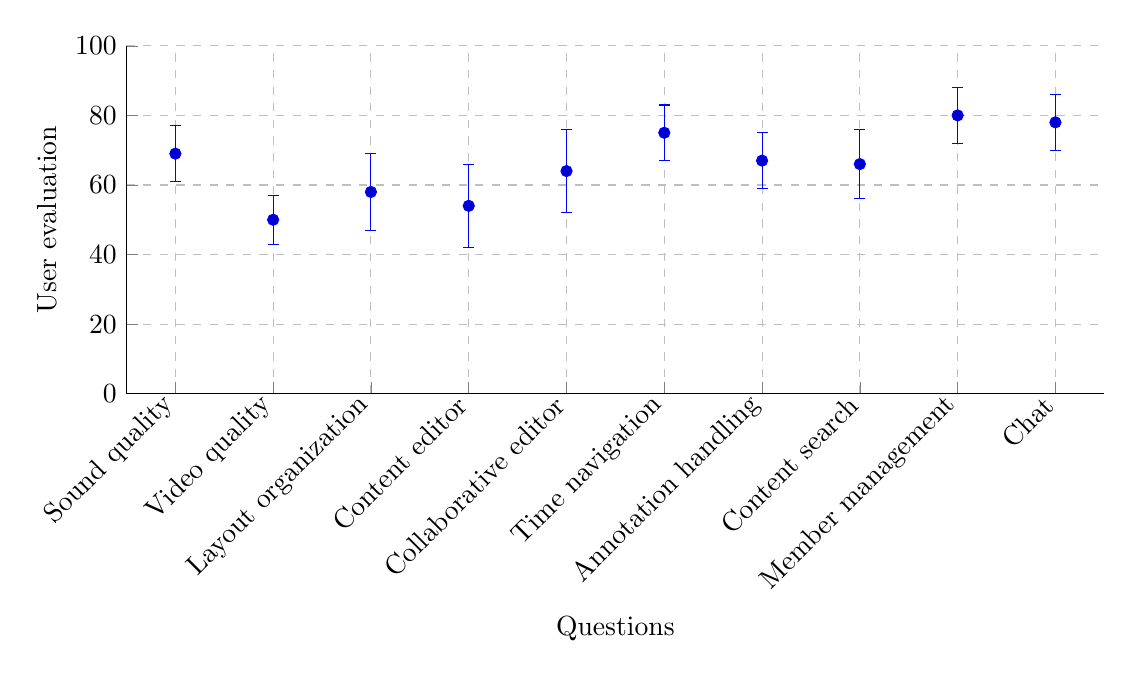
\begin{tikzpicture}[scale=1.0],
\centering
\begin{axis}[
height=6cm,
width=14cm,  
  xlabel={Questions},
  ylabel={User evaluation},
  ymax=100,
  ymin=0,
  xmin=0.5,
  xmax=10.5,
  axis y line*=left,
  axis x line*=bottom,
  xticklabels={Sound quality,Video quality,Layout organization,Content editor,Collaborative editor,Time navigation, Annotation handling, Content search,Member management,Chat},
  xtick={1,...,10},
  ytick={0,20,...,200},
      ymajorgrids=true,
      xmajorgrids=true,
      grid style=dashed,
  x tick label style={rotate=45,anchor=east}]
\addplot+[only marks][error bars/.cd,y dir=both, y explicit]
coordinates {
(1,69) +- (8,8)
(2,50) +- (7,7)
(3,58) +- (11,11)
(4,54) +- (12,12)
(5,64) +- (12,12)
(6,75) +- (8,8)
(7,67) +- (8,8)
(8,66) +- (10,10)
(9,80) +- (8,8)
(10,78) +-(8,8)
};
\addplot[dashed] coordinates {(0,0) (5.5,0)};
\end{axis}
\end{tikzpicture}%